% !TEX root = ../Rulebook.tex
%\newpage
\section{Rotating Table Test}
\label{sec:Rotating Table Test}

The \iaterm{Rotating Table Test}{RTT} introduces moving objects to the competition.
A total of six objects are placed on the rotating table (see Section~\ref{sec:Rotating Table}), of which three must be picked and three are decoy objects.

This requires robots to detect objects and estimate their trajectory in order to grasp them successfully.
To lower the difficulty of this task, the table continously spins with a constant speed, enabling robots to use data from multiple rotations to calculate the optimal grasping position and move their manipulator in time.

%It is explicitly NOT allowed to stop the table (e.g. by pushing the gripper into the table surface).
%
%It is also explicitly NOT allowed to position the gripper in a way that blocks the objects 
%unless it is during the grasping process of a target object and does not affect the table rotation or other objects.

The table starts spinning once the runtime of each team has started.
The initial table rotation is the same for each team to ensure comparability.  

As navigation is not the focus of this test, robots only have to travel to the rotating table and do not have to move to the FINISH location. The run ends once all three objects have been picked or a rule violation has been called by the referees.

See the section \ref{ssec:GraspingObjects} for more detailed information about the grasping process at a Rotating Table.

%
%\paragraph{Purpose and Focus of the Test}
%The purpose of the \iaterm{Rotating Table Test}{RTT} is to assess the robot's ability to manipulate moving objects which are placed on a rotating turntable. The test demands fast perception and manipulation skills in order to pick up objects from a moving surface.
%
%\paragraph{Scenario Environment}
%The same arena as for the Basic Manipulation Test is used. In case that the arena does not already include such a device (see Figure \ref{fig:conveyor_belt}), it will be added only for this particular test.
%
%\begin{figure} [h!]
%	\begin{center}
%%		\subfloat[Conveyor belt]{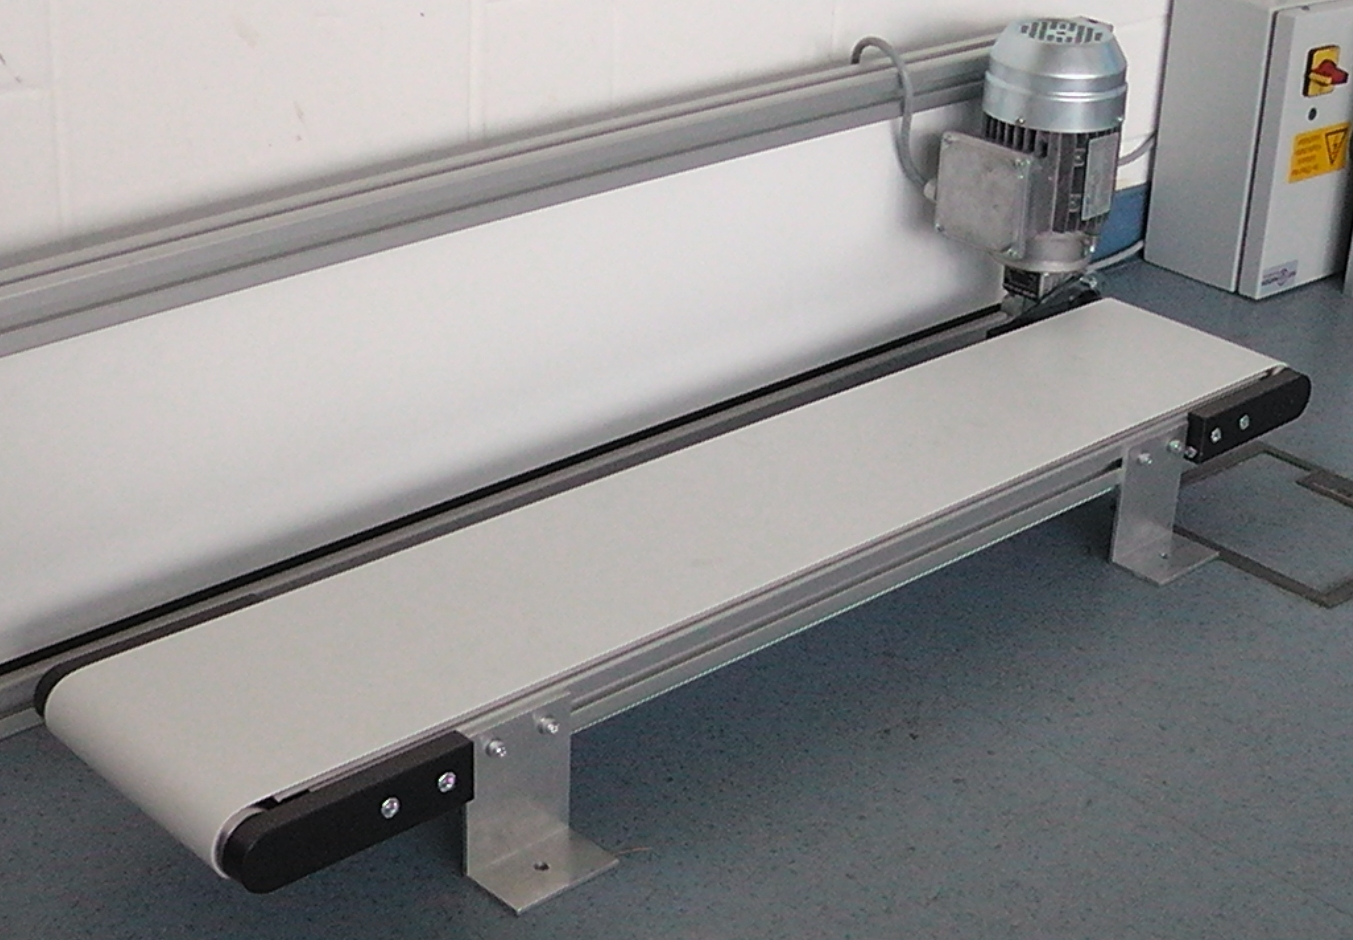
\includegraphics[height = 4cm]{./images/conveyor_belt.jpg}} 
%%		\hspace{1cm}
%		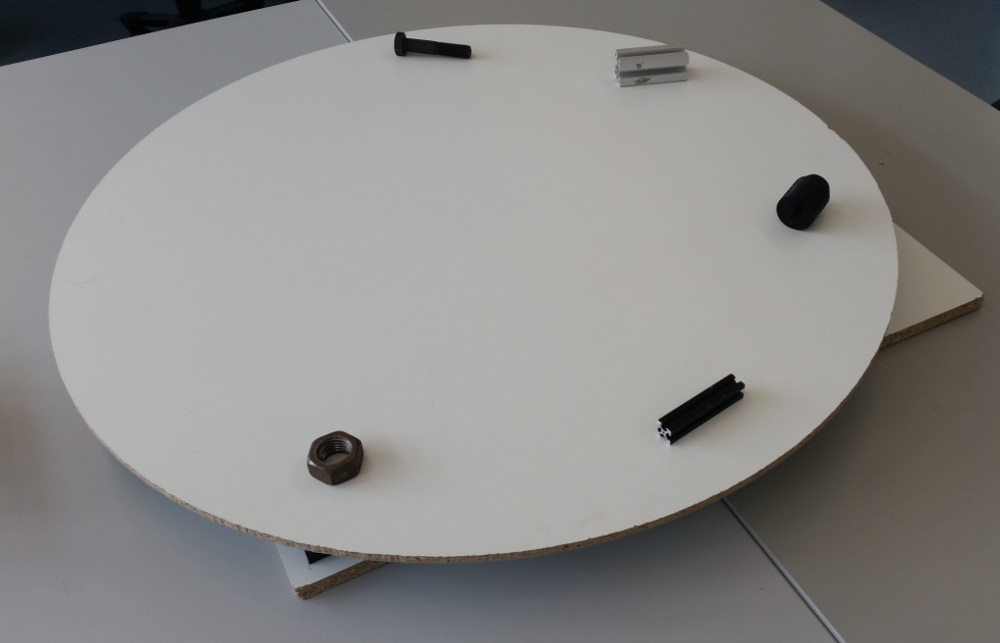
\includegraphics[height = 6cm]{./images/rotating_table.jpg}
%	\end{center}
%	\caption{Illustration of a rotating table used in the competition.}
%	\label{fig:conveyor_belt}
%\end{figure}
%
%
%
%\paragraph{Manipulation Objects}
%The manipulation objects used in this test are defined by the instances described in Table~\ref{tab:Instances}.
%
%\paragraph{Task}
%The task of the robot is to navigate to the location of the rotating table and to grasp all objects from the moving table. The objects can pass multiple times in front of the robot, until the maximum time for the run is over. The robot is supposed to place the grasped objects on the robot itself.
%
%
%%\subsection{Complexity Options}
%%All Complexity Options from BMT apply.
%
%
%%\subsubsection{Speed Complexity (pick one):}
%%
%%\begin{itemize}
%%\item low speed (bonus factor = +0.0): The conveyor belt speed will be not more than 0.5 cm/s
%%\item medium speed (bonus factor = +02):	The conveyor belt speed will be not more than 0.75 cm/s
%%\item high speed (bonus factor = +0.4): The conveyor belt speed will be not more than 0.10 cm/s
%%\end{itemize}
%
%
%
%\paragraph{Rules}
%The following rules have to be obeyed:
%
%\begin{itemize}
%\item A single robot is used.
%\item The robot has to start from outside the arena and to end in the final.
%\item The order in which the teams have to perform will be determined by a draw.
%\item The objects are placed on the rotating table before the run starts by the OC or TC.
%\item The speed of the rotating table is determined by the OC or TC just before the test starts.
%\item The robot will get the task specification from the referee box.
%\item A service area counts as successfully reached as defined in Section~\ref{ssec:Navigating}
%\item A manipulation object counts as successfully grasped as specified in Section~\ref{ssec:PlacingObjects}.
%\item The objects have to be grasped actively from the moving table. The robot is not allowed to stop the items with its gripper.
%\item The run is over when the robot reached the final position or the designated time has expired.
%\item The score for this test will be calculated as defined in \ref{sec:ScoringAndRanking}.
%\end{itemize}
%
%
%
%%
%%\subsection{Scoring}
%%Points are awarded as follows:
%%
%%\begin{itemize}
%%\item 200 points are awarded for successfully grasping an object from the conveyor belt 
%%\item -150 points are given if an object dropped onto the ground, is placed not on the robot itself or dropped from the end of the conveyor..
%%\item -100 points are given if the referees had to switch on the belt manually after signalled by a team member, while a working automatic wireless mechanism to switch it on was available.
%%\item 50 points are awarded if the task has been fully achieved (when all objects placed on the belt are grasped).
%%\end{itemize}
